%% Los cap'itulos inician con \chapter{T'itulo}, estos aparecen numerados y
%% se incluyen en el 'indice general.
%%
%% Recuerda que aqu'i ya puedes escribir acentos como: 'a, 'e, 'i, etc.
%% La letra n con tilde es: 'n.

\chapter{Algoritmos de ordenamiento y mecanismos de manejo referencial}
\label{Algoritmos de ordenamiento y mecanismos del manejo referencial}
Una base de datos relacional esta fuertemente ligada al concepto Entidad Relaci\'on \cite{FBD}(E-R ``Entity Relationship"). Una entidad que representa gr\'aficamente a un concepto del mundo real o abstracta, que da lugar a una tabla en la base de datos. Una relaci\'on entre dos o m\'as entidades describe alguna interacci\'on entre las mismas, el tipo de relaci\'on  dar\'a lugar a un comportamiento entre las entidades involucradas \cite{introbasedatos}.

En un modelo Entidad Relaci\'on (E-R) para base de datos basados en ER Idioms\cite{idioms}, se tiene patrones de dise\~no m\'as definidos, las relaciones que llegan a tener entre entidades y la forma en que se hacen da lugar pr\'acticamente a siguientes siete patrones de dise\~no para un modelo ER.
\begin{enumerate}
\item Una entidad que no hace referencia a otra pero si es referenciada es una entidad de tipo \textit{catalogo}. Act\'ua como un tipificador y generalmente almacenan peque\~nas cantidades de datos, los datos que se almacenan  se conocen a priori y la cantidades de datos son predecibles lo cual no significa que sean estables pueden llegar ha incrementarse, la entidad que hace referencia al \textit{catalogo} llega a ser una entidad de tipo \textit{catalogado}.
\item En algunos casos se tiene entidades que se encuentran sueltas por lo tanto no hacen referencia ni son referenciadas por ninguna otra, la cual es una entidad de tipo \textit{simple}.
\item En un modelo entidad relaci\'on donde una entidad hace referencia a m\'as de una y que su existencia depende de las mismas, a todo este conjunto se le denomina  \textit{composici\'on}, consiste en que puede componer de m\'as de dos incluy\'endose as\'i mismo.
\item
Cuando una entidad es dependiente de la existencia de otra al que detalla es de tipo \textit{detalle} de la alguna entidad maestra, donde el  detalle obedece a la maestra, a diferencia de un catalogador en un maestro no se puede determinar  los posibles datos a priori ni mucho menos estimar la cantidad aproximada de datos que pueda tener y que generalmente almacena cantidades grandes de datos.
\item
Hay veces que una entidad referencia a otra del mismo tipo llegando a ser una relaci\'on recursiva la cual llega a ser una entidad de tipo \textit{reflexivo simple}, cuando se implementa este tipo de relaci\'on es importante tener en cuenta que la relaci\'on no debe ser de obligatoriedad.
\item
En ocasiones es necesario relacionar entidades del mismo tipo y guardar una historia de ellas, la forma de representar este concepto es que una entidad representa la forma que se relacionan la entidad que hace una doble referencia, lo cual lleva a ser una entidad tipo  \textit{reflexivo compuesto}.
\item
Cuando se quiere hacer una especializaci\'on a una entidad en particular esta llega a ser la entidad hija de de la entidad generalizada este tipo de relaci\'on es conocida como \textit{is a} en idioms.
\end{enumerate}

\section{T\'ecnicas de ordenamiento}
En una base de datos las tablas tienen una secuencia de prioridades en el llenado de datos, una manera de obtener esta secuencia es buscar todas las tablas que no tengan ningun \texttt{foreign key}, posteriormente las tablas que tienen como \texttt{foreign key} que referencian a las anteriores que llenamos y asi sucesivamente de manera secuencial, hasta acabar con el ultimo al que no referencia ninguna otra tabla, esto llegar a ser confuso sobre todo si son muchas tablas al momento de hacer el llenado, para lo cual es necesario alguna t'ecnica para el orden correcto del llenado.

La propuesta en este proyecto sobre la t\'ecnica para obtener el orden seg\'un la prioridad en que deben ser llenado las tablas, es identificar primero todas aquellas que son un entidad catalogador, simples y  aquellas que no dependen de ninguna otra en las que puede que en algunos casos pueden estar las entidades maestras  o las que son padres de una generalizaci\'on, los  siguientes a identificar son los catalogados, las que hacen referencia a las identificadas anteriormente pero que estas no deben depender de otras que a\'un no se llen\'o para evitar  tener problemas de inconsistencia. 
\section{Algoritmo de ordenamiento}
\label{Algoritmo de ordenamiento}
Para obtener la lista de tablas seg\'un el orden en que debe ser llenado una base de datos,  es necesario aplicar el siguiente algoritmo:
\begin{enumerate}
\item Crear una matriz bidimensional.
\item Seleccionar las entidades de tipo catalogo, simples, maestras que no dependan de otra entidad y entidades que sean de tipo \textit{reflexivo simple} pero que no hagan referencia a otra distinta de el, para luego almacenar este conjunto en una matriz lineal y que est a su ves agregarlo en la matriz bidimensional.
\item De la matriz bidimensional obtener la \'ultima matriz y por cada elemento buscar todas las entidades que le hagan referencia y agregarlos en un nuevo arreglo lineal, una vez recorrido todos los elementos a\~nadir el arreglo lineal en el arreglo bidimensional.
\item Verificar que se ha recorrido todas las entidades, en caso de que se recorri\'o todo pasar al paso cinco, en caso contrario repetir el paso tres.
\item si se llego hasta aqu\'i es porque ya tenemos un arreglo bidimensional ya con el orden pero esta aun no es la lista para lo que requerimos ya que se da el caso que se pueda repetir mas de una ves el nombre de una entidad en los distintos matrices que contiene la matriz bidimensional por lo tanto es necesario aplicar el algoritmo de ordenaci\'on primeros en ser llenados a la matriz bidimensional.
\end{enumerate}
\section{Aplicaci\'on del algoritmo}
\begin{figure}[H]
\centering
\subfigure{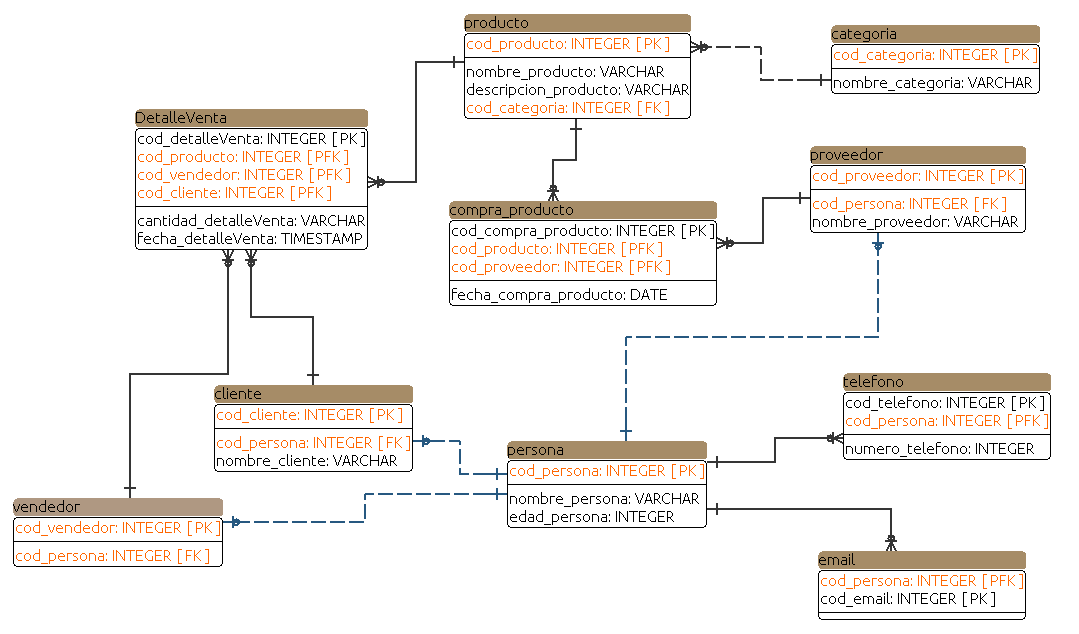
\includegraphics[scale=0.4]{images/modeloER}}
\caption{Modelo ER} 
\floatfoot{\texttt{PFK:} \textit{Primary Foreign Key, llave foranea que a la vez son parte de la llave primaria}\\
\texttt{PK:} \textit{Primary Key, llave primaria}
}
\label{fig:Modelo ER}
\end{figure}
En la Figura \ref{fig:Modelo ER} Modelo ER, podemos observar las distintas entidades de las cuales es necesario identificar las entidades que no hagan referencia aplicando el paso dos del algoritmo podemos identificar una entidad catalogador \emph{categoria} y una entidad que generaliza \emph{persona}, a partir ellas buscamos los que le hacen referencia, \textit{categoria} y \textit{persona} la tomamos como ra\'iz del \'arbol a generar, las entidades que hacen referencia serian \textit{(producto, cliente, vendedor, proveedor, telefono, email)} abajo estar\'ian \textit{(detalleVenta y compra\_producto)} y aplicando el algoritmo se llegar\'ia a la siguiente Figura \ref{fig:ModeloOrdenado} que se encuentra en la p\'agina siguiente.
\begin{figure}[H]
\centering
\subfigure{\includegraphics[scale=0.25]{images/arbol}}
\caption{Modelo Ordenado} \label{fig:ModeloOrdenado}
\end{figure}
\section{Algoritmo de ordenaci\'on \textit{primeros en ser llenado}}
\label{Algoritmo de ordenacion primeros en ser llenado}
Para obtener una lista ordenada de acuerdo al orden que se debe realizar el llenado, se inicia el recorrido de las matrices que trae la matriz bidimensional obtenida del algoritmo anterior, porque si recordamos la lista se orden\'o seg\'un a que una entidad no dependiera de otra entidad, al recorrer podemos encontrarnos que una entidad se repite en distintos lugares, al  inicio de la matriz bidimensional, puede tambi\'en estar listada en medio o al final incluso se puede dar el caso que en uno de las matrices se repita m\'as de una vez. Si vemos la Figura \ref{fig:ModeloOrdenado} la entidad \textit{detalleVenta} se repite m\'as de una vez en la misma fila.

Entonces cual lo tomamos como v\'alido?.
Para lo cual el  recorrido se comienza con el \'ultimo de las matrices que tiene la matriz bidimensional, una vez encontrada las dem\'as que puedan encontrarse en posteriores no llegar\'a a ser v\'alida porque si bien hizo una referencia a un principio ser\'a valida el \'ultimo. Esto se justifica porque si se encuentra al \'ultimo es porque a\'un hace referencia a alg\'un elemento de la matriz anterior al que pertenece, por lo tanto se debi\'o esperar que se llegue hasta ese punto. para el caso de la Figura \ref{fig:ModeloOrdenado} listamos el \'ultimo evitando que se repita.
Para obtener una correcta lista ordenada seg\'un el orden en que deben ser llenados es necesario seguir la siguiente secuencia de pasos:
\begin{enumerate}
\item Crear un matriz de tama\~no de la cantidad de entidades de la base de datos seleccionada.
\item obtener la \'ultima matriz de la matriz bidimensional.
\item Recorrer la matriz y verificar por cada elemento no exista en la matriz del paso uno, en caso de que no exista a\~nadir, en caso de que si no a\~nadir y pasar a la siguiente elemento.
\item Eliminar la \'ultima matriz de la matriz bidimensional.
\item Si existen mas matrices en la matriz bidimensional volver a repetir el paso dos, caso contrario pasar al siguiente paso.
\item Invertir el orden de la matriz del paso uno.
\item Retornar la matriz creado en el paso uno que llegar\'ia a ser el orden que se requiere.
\end{enumerate}
\section{Aplicaci\'on del algoritmo de \textit{primeros en ser llenado}}
Con el algoritmo llegamos a tener el siguiente orden en que debe ser llenado para el ejemplo dado en la figura  \ref{fig:Modelo ER}.
\begin{figure}[H]
\centering
\subfigure{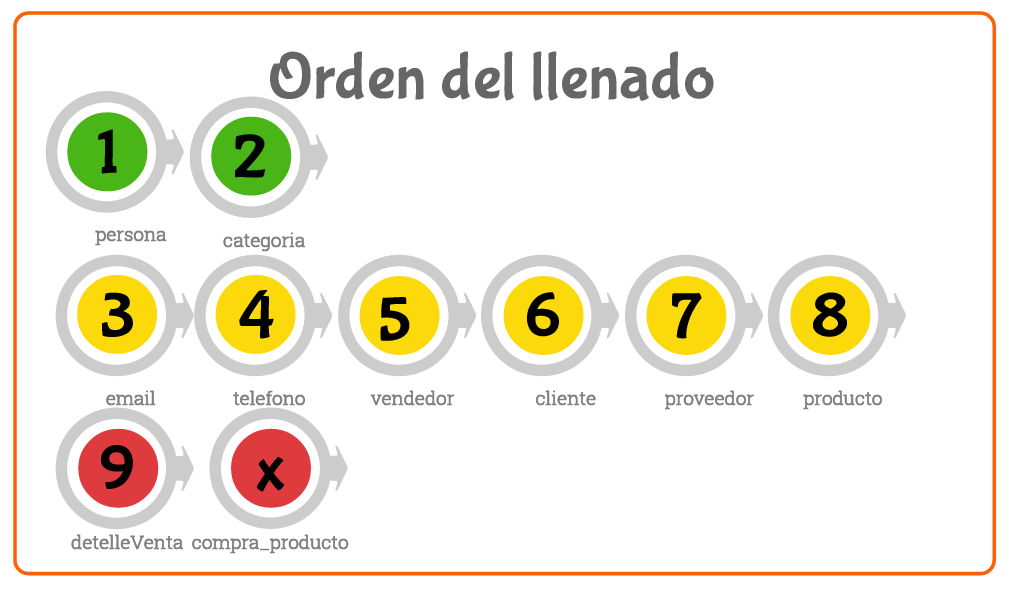
\includegraphics[scale=0.38]{images/ordenCorrecto}}
\caption{Orden de llenado}
\label{fig:Orden de llenado}
\end{figure}
El orden a seguir para este ejemplo es iniciar por el color verde terminando en el color rojo, el orden en cada fila no influye en el resultado permitiendo as\'i la flexibilidad de tomar cualquier elemento para el inicio de cada fila o el conjunto de elementos del mismo color.
\section{Mecanismo de \textit{manejo de referencial} de una base de datos}
Cuando un modelo entidad relaci\'on es llevado a un sistema gestor de base de datos, donde por cada entidad se crea una tabla y las  referencias son representadas mediante las llaves primarias y llaves for\'aneas, En caso de un modelo entidad relaci\'on basado en ER Idioms tiene ciertas caracter\'isticas que son.
\subsection{Llaves primarias compuestas (\texttt{composite keys})}
Cuando se tiene m\'as de un \texttt{primary key}, entre ellas las que son propias de la tabla y otras pertenecientes a las que referencia que vienen como primarias, llegan a formar parte del \texttt{primary key} de la tabla, formando as'i \texttt{composite keys} para la misma. En conceptos de entidad relaci\'on en la figura  \ref{fig:llaves compuestas} se puede observar  las entidades que hacen referencia a otra.
\begin{figure}[H]
\centering
\subfigure{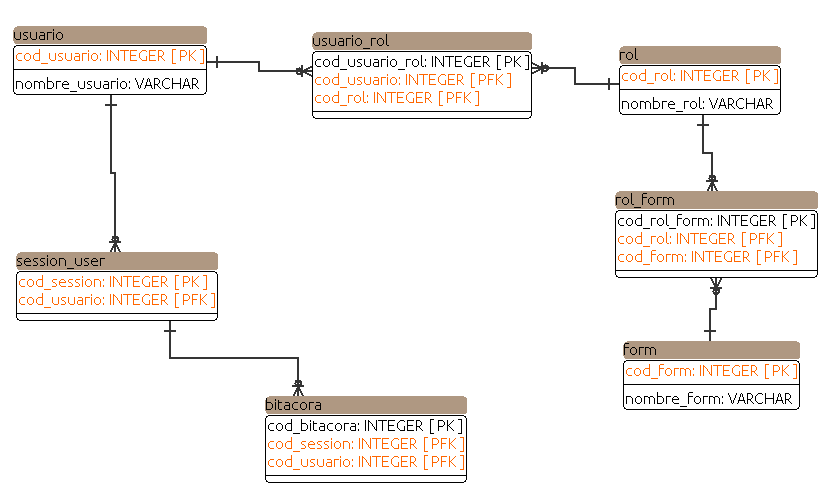
\includegraphics[scale=0.5]{images/llavesCompuestas}}
\floatfoot{\texttt{PFK:} \textit{Primary Foreign Key, llave foranea que a la vez son parte de la llave primaria}\\
\texttt{PK:} \textit{Primary Key, llave primaria}}
\caption{Llaves compuestas} \label{fig:llaves compuestas}
\end{figure}
Donde se puede ver que la entidad \textit{usuario\_rol} hace referencia a las entidades \textit{usuario} y \textit{rol}, las tres entidades llegar\'ian a formar una composici\'on  (\textit{usuario\_rol} compone de \textit{usuario} y \textit{rol}) donde la existencia de \textit{usuario\_rol} es dependiente de las que compone. Si este modelo lo llevamos a un gestor de base de datos un DBMS se llega a tener como en la figura \ref{SQLtablaUsuarioRolComposite}.\\
\lstset{language=sql,breaklines=true}
\label{SQLtablaUsuarioRolComposite}
\captionof{lstlisting}{SQL tabla usuario\_rol}
\begin{lstlisting}
CREATE TABLE usuario_rol(
  cod_usuario_rol serial NOT NULL,
  cod_usuario INTEGER NOT NULL,
  cod_rol INTEGER NOT NULL,
  CONSTRAINT cod_usuario_rol PRIMARY KEY (cod_usuario_rol,cod_usuario,cod_rol),
  CONSTRAINT rol_usuario_rol_fk FOREIGN KEY (cod_rol)
      REFERENCES rol (cod_rol) MATCH SIMPLE
      ON UPDATE NOT ACTION ON DELETE NOT ACTION,
  CONSTRAINT usuario_usuario_rol_fk FOREIGN KEY (cod_usuario)
      REFERENCES usuario (cod_usuario) MATCH SIMPLE
      ON UPDATE NOT ACTION ON DELETE NOT ACTION
)
\end{lstlisting}
El \texttt{primary key} propia es independiente en cambio \textit{cod\_usuario} es perteneciente a la tabla \textit{usuario} pero viene como \texttt{primary key} lo mismo sucede con el campo \textit{cod\_rol}  que pertenece a la tabla \textit{rol}, como ambas \texttt{foreing key} vienen como \texttt{primary key} la tabla \textit{usuario\_rol} llegar'ia a tener un \texttt{primary key} compuesta de tres \textit{cod\_usuario\_rol, cod\_usuario, cod\_rol}. Cuando se quiere hacer una inserci\'on de un registro a la tabla \textit{usuario\_rol} sin antes haber realizado una inserci\'on a las tablas de \textit{usuario} y \textit{rol} cualquier DBMS no lo realiza la inserci\'on por razones de primero debe existir datos en las tablas.
\subsection{Mejor uso de Join}
Al hacer uso de llaves compuestas(\texttt{composite keys}) hace que un identificador llegue m\'as all\'a de lo que normalmente se acostumbra veamos en la figura  \ref{fig:llavesCompuestas}.\\
\begin{figure}[H]
\centering
\subfigure{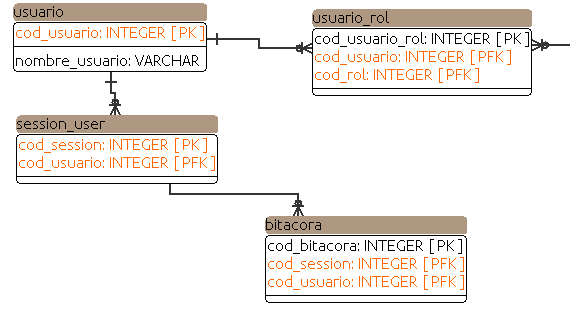
\includegraphics[scale=0.4]{images/join}}
\caption{Modelo E-R con llaves compuestas} \label{fig:llavesCompuestas}
\floatfoot{\texttt{PFK:} \textit{Primary Foreign Key, llave foranea que a la vez son parte de la llave primaria}\\
\texttt{PK:} \textit{Primary Key, llave primaria}}
\end{figure}
Donde en la entidad bit\'acora se tiene tres \texttt{primary key} llegando a ser una llave compuesta(\texttt{composite key}) y una de ellas es \textit{cod\_usuario} que si bien viene de \textit{session\_user} realmente su origen es en \textit{usuario}, por lo tanto podemos hacer un join entre \textit{bitacora} y \textit{usuario} evitando hacerlo con \textit{session\_user} obteniendo asi una consulta mas eficiente.
\section{Mecanismo de referenciaci\'on}
Cuando generamos datos de prueba para una base de datos es importante tener en cuenta el manejo de las llaves compuestas(\texttt{composite keys}), no podemos generar al azar los \texttt{foreign key} porque se llegar'ia a tener problemas de inconsistencia.

Una t\'ecnica para evitar los problemas de inconsistencia es tener como fuente la tabla al que se referencia y los atributos  tomarlo como base para la generaci\'on de \emph{n} datos.
\subsection{Referencia simple}
Las referencias simples son cuando una tabla recibe solo un \texttt{primary key} o \texttt{foreign key} por parte de otra, observemos la figura \ref{SQLUsuarioRolSimple}.
\lstset{language=sql,breaklines=true}
\label{SQLUsuarioRolSimple}
\captionof{lstlisting}{Referencia simple}
\begin{lstlisting}
CREATE TABLE usuario_rol(
  cod_usuario_rol serial NOT NULL,
  cod_usuario INTEGER NOT NULL,
  cod_rol INTEGER NOT NULL,
  CONSTRAINT cod_usuario_rol PRIMARY KEY (cod_usuario_rol,cod_usuario,cod_rol),
  CONSTRAINT rol_usuario_rol_fk FOREIGN KEY (cod_rol)
      REFERENCES rol (cod_rol) MATCH SIMPLE
      ON UPDATE NOT ACTION ON DELETE NOT ACTION,
  CONSTRAINT usuario_usuario_rol_fk FOREIGN KEY (cod_usuario)
      REFERENCES usuario (cod_usuario) MATCH SIMPLE
      ON UPDATE NOT ACTION ON DELETE NOT ACTION
)
\end{lstlisting}
En la figura \ref{SQLUsuarioRolSimple} se puede observar el c\'odigo  \texttt{SQL} (por sus siglas en ingl\'es Structured Query Language) de la tabla \textit{usuario\_rol} de la figura \ref{fig:llaves compuestas}.  La tabla mencionada esta conformada de dos llaves que no son propias de la misma, \textit{cod\_usuario} forma parte de la tabla \textit{usuario} y \textit{cod\_rol} apunta a la tabla \textit{rol}, ambos son campos que apuntan a su respectiva tabla de manera \'unica por lo tanto se deja entender que se hace una referencia simple de llaves.
\subsection{Referencia compuesta}
Las referencias compuestas son cuando una tabla recibe m\'as de un \texttt{primary key} o \texttt{foreign key} por parte de otra. Es importante tomar los atributos que apuntan a otra como un conjunto de atributos para manejar como base para la generaci\'on de los datos requeridos.
\lstset{language=sql,breaklines=true}
\label{lst:SQLReferenciaCompuesta}
\captionof{lstlisting}{Referencia compuesta}
\begin{lstlisting}
CREATE TABLE bitacora(
  cod_bitacora serial NOT NULL,
  cod_session INTEGER NOT NULL,
  cod_usuario INTEGER NOT NULL,	  
  CONSTRAINT bitacora_pk PRIMARY KEY (cod_bitacora,cod_session,cod_usuario),
  CONSTRAINT session_user_bitacora_fk FOREIGN KEY (cod_session,cod_usuario)
      REFERENCES "session_user" (cod_session,cod_usuario) MATCH SIMPLE
      ON UPDATE NOT ACTION ON DELETE NOT ACTION
)
\end{lstlisting}
En la figura \ref{lst:SQLReferenciaCompuesta} el campo \textit{cod\_session} y \textit{cod\_usuario} de la tabla \textit{bitacora} hace referencia a \textit{session\_user} a los campos \textit{cod\_session} y \textit{cod\_usuario}, son dos campos que apuntan a la misma tabla que este caso \textit{session\_user} por lo tanto llegar\'ia a ser una referencia compuesta.